\section{问题二：无泄漏预测与分位鲁棒调度}
\subsection{滚动预测}
从2025年1月1日起连续推进SOC，1月作为预测与状态热身期，正式统计从2月1日开始。对变量$x\in\{L,G,\pi\}$，同一时段的点预测为
\begin{equation}\hat x_{d,t}=0.65\,\operatorname{med}\{x_{j,t}:j<d,\ j\equiv d\pmod 7\}+0.35\,\operatorname{med}\{x_{j,t}:d-7\le j<d\}.\label{eq:forecast}\end{equation}
同星期部分最多取最近4个同星期样本。负荷预测MAE和WAPE分别为324.10 kW和7.01\%；光伏分别为203.79 kW和8.82\%。图~\ref{fig:predexample}展示一日预测实例。
\begin{figure}[H]\centering
\includegraphics[width=0.92\textwidth]{../figures/fig04_prediction_example.pdf}
\caption{负荷与光伏历史滚动预测示例}\label{fig:predexample}\end{figure}
\subsection{安全裕度与优化}
将历史28日内有效预测残差$u_{j,t}=n_{j,t}-\hat n_{j,t}$的80\%分位记为$\rho_{d,t}$，以
\begin{equation}\tilde n_{d,t}=\hat n_{d,t}+\rho_{d,t}\label{eq:robustnet}\end{equation}
代入问题一的线性规划。实际供给不足部分
\begin{equation}e_{d,t}=\max\{n_{d,t}-(g_{d,t}+q_{d,t}-c_{d,t}),0\}\end{equation}
按$5\pi_{d,t}$结算。该模型是场景风险模型的线性分位近似，代码并未计算CVaR尾部值，故本文不将结果表述为完整CVaR优化。
\subsection{结果}
334日累计费用为15,386,\allowbreak 279.80元，紧急购电为427,890.01 kWh。与使用事后真实负荷和光伏的完美信息下界相比，本结果强调可实施性：任一决策时刻均不读取未来实测值，且日末SOC直接传递至下一日。
\begin{figure}[H]\centering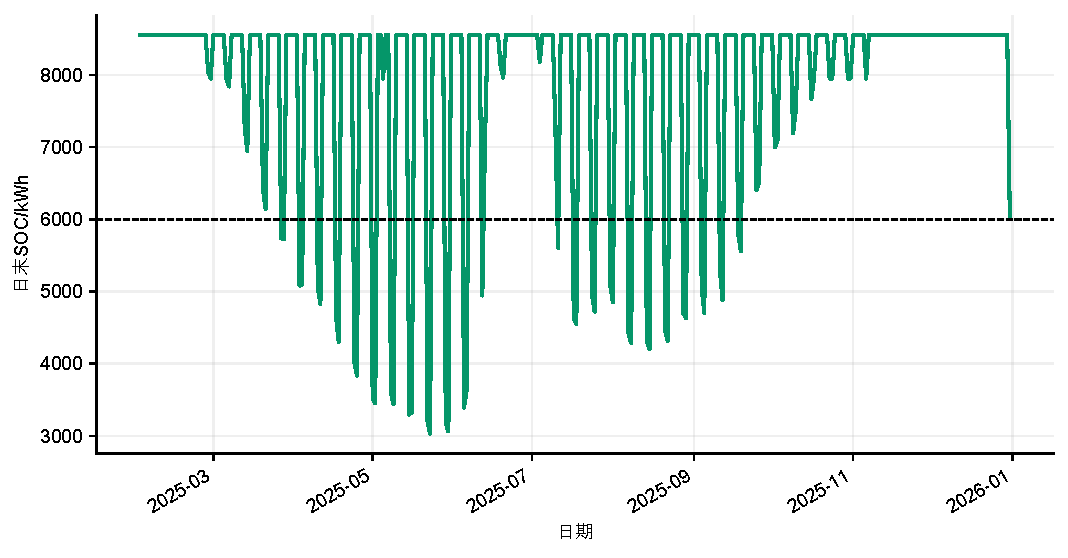
\includegraphics[width=0.92\textwidth]{../figures/fig07_crossday_soc.pdf}
\caption{正式统计期内储能日初与日末SOC连续轨迹}\label{fig:crossdaysoc}\end{figure}
图~\ref{fig:crossdaysoc}显示SOC并未在月初或每日被人为重置，这保证了334日费用来自一条连续可执行的状态路径。
